\documentclass[crop, tikz]{standalone}
\usepackage{tikz}
\usetikzlibrary{arrows.meta}

\begin{document}
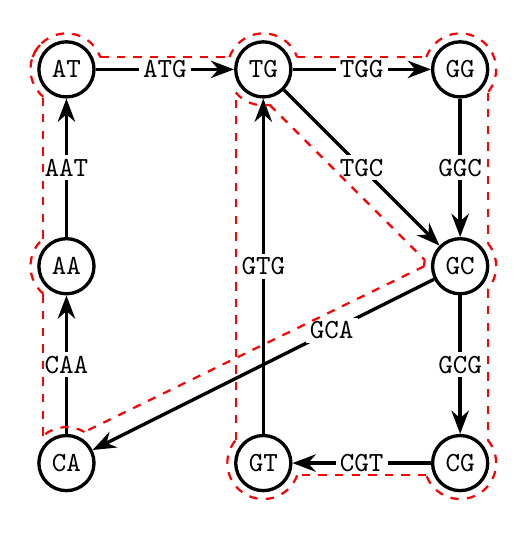
\begin{tikzpicture}[
  >=Stealth,
  font=\tt,
  vtx/.style={circle, draw, very thick, minimum size=7mm, inner sep=1pt},
  lbl/.style={fill=white, inner sep=1.5pt},
  tour/.style={thick, red, dashed},
]
  \foreach \name/\x/\y in {AT/0/5, TG/2.5/5, GG/5/5, GC/5/2.5, CG/5/0, GT/2.5/0, CA/0/0, AA/0/2.5}
    \node[vtx] (\name) at (\x, \y) {\name};

  \foreach \from/\to/\lab/\pp in {%
      AT/TG/ATG/.5, TG/GG/TGG/.5, GG/GC/GGC/.5, GC/CG/GCG/.5, CG/GT/CGT/.5,
      GT/TG/GTG/.5, TG/GC/TGC/.5, GC/CA/GCA/.3, CA/AA/CAA/.5, AA/AT/AAT/.5}
    \draw[->, very thick] (\from) -- node[lbl, pos=\pp] {\lab} (\to);

  % dashed Eulerian tour: arcs around nodes joined by straight segments
  % connecting each arc's end (b<i>) to the next arc's start (a<i+1>)
  \foreach \name/\sa/\ea [count=\i] in {%
      AT/-200/-340, TG/-200/-340, GG/-200/-400, GC/-320/-400, CG/-320/-520,
      GT/-380/-580, TG/-500/-440, GC/-550/-540, CA/-660/-590, AA/-490/-590, AT/-490/-590}
    \draw[tour] (\name) ++(\sa:13pt) coordinate (a\i) arc (\sa:\ea:13pt) coordinate (b\i);

  \foreach \i [evaluate=\i as \j using {int(\i + 1)}] in {1, ..., 10}
    \draw[tour, rounded corners=3mm] (b\i) -- (a\j);
\end{tikzpicture}
\end{document}
